\chapter{MARCO TEÓRICO}
\label{cap:teorico}

El descubrimiento de clases novedosas en nubes de puntos de patrimonio
arquitectónico es un tema interdisciplinario que abarca diversas áreas. Este
marco teórico se organiza en tres secciones: conceptos de ingeniería civil
aplicados a la documentación del patrimonio, computación y algoritmos empleados
para el procesamiento de nubes de puntos y métricas de evaluación del modelo.

% =====================================================================
\section{Ingeniería Civil y Conservación del Patrimonio}

La ingeniería civil aporta el objeto de estudio y los criterios de
documentación. A continuación se presentan los conceptos de esta disciplina que
son relevantes para este trabajo.

\subsection{Nube de Puntos}

Una nube de puntos es un conjunto $P=\{(x_i,f_i)\}_{i=1}^{N}$ donde
$x_i\in\mathbb{R}^3$ es la posición medida de un punto de la superficie y $f_i$
los atributos que registra el sensor, en este caso color y normal. No tiene
conectividad ni orden: es una lista de mediciones, no una malla.

\subsection{Levantamiento Láser Terrestre (TLS)}

El levantamiento láser terrestre es el registro de una edificación mediante un
escáner estacionado en posiciones fijas. Es el formato en que la Facultad de
Ingeniería Civil entrega el levantamiento de la Catedral de Lima y la fuente de
datos de este trabajo.

\subsection{Voxelización}

La voxelización divide el espacio en cubos de lado fijo y sustituye por un único
representante todos los puntos que caen en un mismo cubo. Reduce el número de
puntos y homogeniza la densidad. El lado del cubo se denomina tamaño de vóxel.

\subsection{Sección Espacial}

Una sección es una partición espacial disjunta del levantamiento: nave, coro,
ábside, torres y fachada. Es la unidad indivisible de trabajo del proyecto, ya
que ninguna etapa requiere la nube completa en memoria y ninguna sección depende
de otra.

\subsection{Segmentación Semántica}

La segmentación semántica asigna una etiqueta de clase a cada punto de $P$. Se
distingue de la segmentación de instancias, que además separa objetos distintos
de una misma clase y que queda fuera del alcance de este trabajo.

\subsection{Clase Conocida y Clase Novedosa}

$\mathcal{C}_k$ es el subconjunto de clases con puntos etiquetados durante el
entrenamiento y $\mathcal{C}_n$ el de clases presentes en la nube pero sin
ninguna etiqueta, con $\mathcal{C}_k\cap\mathcal{C}_n=\emptyset$ y
$\mathcal{C}=\mathcal{C}_k\cup\mathcal{C}_n$. En patrimonio, $\mathcal{C}_n$
recoge los elementos singulares de cada edificio, que no figuran en ningún
catálogo previo.

% =====================================================================
\section{Computación y Algoritmos}

La computación y los algoritmos son las herramientas para procesar y analizar
las nubes de puntos. Aquí se presentan los conceptos y técnicas que intervienen
en el modelo propuesto.

\subsection{Descubrimiento de Clases Novedosas (NCD)}

El NCD consiste en producir una asignación $\hat{y}:P\rightarrow\mathcal{C}$
correcta sobre $\mathcal{C}_k$ y consistente sobre $\mathcal{C}_n$, entendiendo
por consistente que los puntos de una misma clase novedosa reciban la misma
etiqueta, aunque esa etiqueta no tenga nombre. Es la capacidad de detectar
formas nuevas sin haberlas visto etiquetadas.

\subsection{Descriptor de Punto}

Un descriptor es el vector numérico asociado a un punto o a una región que
resume su contenido. HyperNCD~\cite{zhang2026hyperncd} describe cada punto
mediante la concatenación de dos componentes:
\begin{equation}
F_i=\left[f_{\mathrm{sem}}(x^i);\,f_{\mathrm{geo}}(x^i)\right].
\label{eq:hyperncd3}
\end{equation}

\subsubsection{Descriptor Semántico}

Salida por punto de la red troncal supervisada de HyperNCD, una
MinkowskiUNet-34C de 96 canales. Codifica a qué se parece un punto en términos
de las clases que la red vio etiquetadas. Se denota $f_{\mathrm{sem}}$.

\subsubsection{Descriptor Geométrico Analítico}

Vector calculado con una fórmula cerrada, sin aprendizaje, a partir de los
autovalores de la matriz de covarianza de un vecindario local de $k=15$ vecinos:
linealidad, planaridad y dispersión, concatenados en la implementación con el
centroide de la región, lo que da una dimensión total de 6. Se denota
$f_{\mathrm{geo}}$ y es el componente que este trabajo sustituye.

\subsubsection{Descriptor Auto-supervisado}

Salida del codificador PTv3 preentrenado de Sonata~\cite{wu2025sonata}, usado
con pesos congelados. Su dimensión es 1088, resultado de concatenar las anchuras
$512+384+192$ de las tres últimas etapas durante la propagación inversa del
submuestreo. Se denota $f_{\mathrm{ssl}}$ y codifica estructura aprendida sobre
140 mil escenas, sin haber visto las clases de este proyecto.

\subsection{Aprendizaje Auto-supervisado}

Régimen de entrenamiento en el que la señal de supervisión se construye a partir
de los propios datos, por ejemplo vistas distintas de una misma escena que deben
producir representaciones parecidas, y no de etiquetas humanas.

\subsection{Codificador Congelado}

Red cuyos pesos no se actualizan y que se usa exclusivamente en inferencia. Su
costo se paga una sola vez y no en cada época, lo que permite calcular su salida
por adelantado y almacenarla en disco.

\subsection{Atajo Geométrico}

Modo de falla del preentrenamiento auto-supervisado en tres dimensiones,
diagnosticado por Sonata: la representación colapsa sobre pistas geométricas
fácilmente accesibles, como la normal, la altura o la curvatura local, en lugar
de aprender semántica. Es la razón por la que $f_{\mathrm{geo}}$ resulta
cuestionable como base de un razonamiento semántico.

\subsection{Serialización}

Ordenamiento de los puntos mediante una curva de llenado de espacio, de tipo Z o
Hilbert, de modo que la proximidad en $\mathbb{R}^3$ se traduzca en proximidad
dentro de una secuencia unidimensional. Es el mecanismo que permite a PTv3
aplicar atención con costo lineal.

\subsection{Rejilla Dispersa}

Estructura de datos de MinkowskiEngine en la que los puntos se indexan por
coordenada entera de vóxel y solo se almacenan los vóxeles ocupados. Es la
estructura sobre la que opera $f_{\mathrm{sem}}$.

\subsection{Propagación Inversa del Submuestreo}

También llamada \emph{up-cast}, devuelve las características del codificador a
la resolución de entrada reutilizando los índices de agrupamiento que el propio
submuestreo registró. Es necesaria porque el codificador entrega su salida
submuestreada varias veces.

\subsection{Prototipo}

Vector $P_k\in\mathbb{R}^{C}$ que actúa como representante de un grupo de puntos
o regiones semejantes. El número de prototipos $K$ se fija igual al número de
clases del conjunto. La pertenencia de cada punto se expresa mediante una matriz
de asignación suave $S_p$, cuyo elemento $s_{i,k}$ indica con qué peso el punto
$i$ pertenece al prototipo $k$.

\subsection{Región o Superpunto}

Agrupación de puntos vecinos y semejantes que el método trata como una sola
unidad. El razonamiento de HyperNCD opera sobre regiones y no sobre puntos, lo
que reduce el número de nodos en varios órdenes de magnitud.

\subsection{Hipergrafo}

Estructura $\mathcal{H}=(\mathcal{V},\mathcal{E})$ en la que una arista puede
conectar más de dos nodos a la vez. Frente a un grafo ordinario, restringido a
relaciones binarias, permite expresar que varias clases conocidas concurren
simultáneamente en la explicación de una novedosa.

\subsubsection{Hiperarista}

Elemento $e_i\in\mathcal{E}$ formado por un prototipo $P_i$ y sus $M$ prototipos
más afines. El valor $M=8$ es el reportado como óptimo por los autores de
HyperNCD.

\subsubsection{Afinidad entre Prototipos}

Medida de semejanza entre dos prototipos, combinación convexa de una componente
geométrica $S_g$ y una semántica $S_s$:
\begin{equation}
S_b=\alpha\,S_g+(1-\alpha)\,S_s,\qquad \alpha\in[0,1].
\label{eq:afinidad}
\end{equation}
$S_g$ es un núcleo gaussiano de temperatura $\tau=0{,}1$ sobre el descriptor
geométrico y $S_s$ una similitud por coseno sobre el semántico.

\subsection{Pseudo-etiqueta}

Etiqueta que el propio modelo asigna a un punto sin supervisión humana y que
después usa como si fuera verdadera para continuar entrenando. Un suavizado de
parámetro $\epsilon=0{,}15$ reduce el sobreajuste durante su generación.

\subsection{Normalización de Sinkhorn-Knopp}

Procedimiento de normalización iterativa de una matriz que fuerza a que sus
filas y columnas sumen valores prefijados. HyperNCD lo emplea para repartir las
pseudo-etiquetas de forma equilibrada entre clases y evitar que todos los puntos
caigan en una sola.

% =====================================================================
\section{Métricas de Evaluación de Modelos}
\label{sec:metricas}

Para evaluar la efectividad del modelo se utilizan las métricas siguientes. El
criterio de reporte es explícito: una métrica no se presenta como un número
aislado, sino junto a la expresión que la define, al número de variables que
promedia y a la identificación de cuál de ellas domina el valor agregado.

\subsection{Intersection over Union (IoU)}

Para una clase $c$, la intersección sobre unión se define como:
\begin{equation}
\mathrm{IoU}_c=\frac{TP_c}{TP_c+FP_c+FN_c},
\label{eq:iou}
\end{equation}
donde $TP_c$, $FP_c$ y $FN_c$ son los puntos verdaderos positivos, falsos
positivos y falsos negativos de esa clase.

\subsection{IoU Media (mIoU)}

La métrica agregada es el promedio de la anterior sobre un conjunto de clases:
\begin{equation}
\mathrm{mIoU}(\mathcal{S})=\frac{1}{|\mathcal{S}|}\sum_{c\in\mathcal{S}}\mathrm{IoU}_c,
\qquad
\mathcal{S}\in\{\mathcal{C}_k,\;\mathcal{C}_n,\;\mathcal{C}\}.
\label{eq:miou}
\end{equation}
Se reporta por separado como mIoU \emph{known}, mIoU \emph{novel} y mIoU
\emph{all}.

\subsection{Análisis de Dominancia}

La Ec.~\eqref{eq:miou} es una media aritmética no ponderada, de modo que
\begin{equation}
\frac{\partial\,\mathrm{mIoU}}{\partial\,\mathrm{IoU}_c}=\frac{1}{|\mathcal{S}|}
\qquad \forall\, c\in\mathcal{S}.
\label{eq:dominancia}
\end{equation}
Cada clase pesa igual con independencia de su número de puntos. Por ello el
valor agregado se acompaña siempre de la clase dominante:
\begin{equation}
c^{*}=\arg\max_{c\in\mathcal{S}}\bigl|\mathrm{IoU}_c-\mathrm{mIoU}(\mathcal{S})\bigr|.
\label{eq:dominante}
\end{equation}

\subsection{Emparejamiento Húngaro}

Como las clases de $\mathcal{C}_n$ se descubren sin etiqueta, la correspondencia
entre agrupaciones predichas y clases reales se resuelve por asignación óptima:
\begin{equation}
\sigma^{*}=\arg\max_{\sigma\in\mathfrak{S}_{|\mathcal{C}_n|}}
\sum_{c\in\mathcal{C}_n}\mathrm{IoU}\bigl(\hat{y}=\sigma(c),\;y=c\bigr).
\label{eq:hungaro}
\end{equation}

\subsection{Índice de Rand Ajustado (ARI)}

Mide la coincidencia entre la agrupación descubierta y la real con independencia
del emparejamiento:
\begin{equation}
\mathrm{ARI}=
\frac{\sum_{ij}\binom{n_{ij}}{2}
-\Bigl[\sum_i\binom{a_i}{2}\sum_j\binom{b_j}{2}\Bigr]\big/\binom{n}{2}}
{\tfrac{1}{2}\Bigl[\sum_i\binom{a_i}{2}+\sum_j\binom{b_j}{2}\Bigr]
-\Bigl[\sum_i\binom{a_i}{2}\sum_j\binom{b_j}{2}\Bigr]\big/\binom{n}{2}},
\label{eq:ari}
\end{equation}
donde $n_{ij}$ es el número de puntos comunes entre la agrupación $i$ y la clase
$j$, y $a_i$ y $b_j$ sus marginales.

\subsection{Información Mutua Normalizada (NMI)}

Complementa al ARI midiendo la información que una agrupación aporta sobre la
otra:
\begin{equation}
\mathrm{NMI}(U,V)=\frac{2\,I(U;V)}{H(U)+H(V)},
\label{eq:nmi}
\end{equation}
donde $I$ es la información mutua y $H$ la entropía.

\subsection{Linear Probing}

Protocolo de evaluación de un descriptor congelado: se entrena únicamente un
clasificador lineal $W$ sobre él,
\begin{equation}
\hat{y}_i=\arg\max\left(W^{\top}f_{\mathrm{ssl}}(x^i)+b\right),
\label{eq:probe}
\end{equation}
de modo que el desempeño resultante queda atribuido a la representación y no al
clasificador.

\subsection{Ganancia Absoluta}

Diferencia de mIoU sobre las clases novedosas entre el modelo híbrido y la línea
base:
\begin{equation}
\Delta\mathrm{mIoU}^{\mathrm{novel}}=
\mathrm{mIoU}^{\mathrm{novel}}_{\mathrm{hib}}-\mathrm{mIoU}^{\mathrm{novel}}_{\mathrm{base}}.
\label{eq:delta}
\end{equation}

\subsection{Brecha Cerrada}

La ganancia absoluta no es interpretable por sí sola, porque el techo alcanzable
depende de la sección. Esta métrica, propuesta en el presente trabajo, la
normaliza por la brecha que separa a la línea base de su propio desempeño sobre
las clases que sí vio etiquetadas:
\begin{equation}
G=\frac{\mathrm{mIoU}^{\mathrm{novel}}_{\mathrm{hib}}-\mathrm{mIoU}^{\mathrm{novel}}_{\mathrm{base}}}
{\mathrm{mIoU}^{\mathrm{known}}_{\mathrm{base}}-\mathrm{mIoU}^{\mathrm{novel}}_{\mathrm{base}}}.
\label{eq:G}
\end{equation}
$G$ es adimensional: $G=0$ indica que la sustitución no aporta, $G=1$ que las
clases novedosas alcanzan la calidad con que el modelo segmenta las conocidas y
$G<0$ degradación.

\subsection{Atribución por Etapas}
\label{sec:metricas-hibrido}

Como el proceso es separable en dos etapas, la métrica se reporta también en el
punto intermedio y no solo al final: \emph{linear probing} sobre el descriptor
(Ec.~\eqref{eq:probe}) antes de la formación de prototipos y mIoU
(Ec.~\eqref{eq:miou}) después. Esa separación permite atribuir una mejora a la
representación o al razonamiento, y no al sistema tratado como caja negra.

% =====================================================================
\section{Diseño de la Tesis}
\label{sec:diseno-teorico}

\begin{figure}[H]
\centering
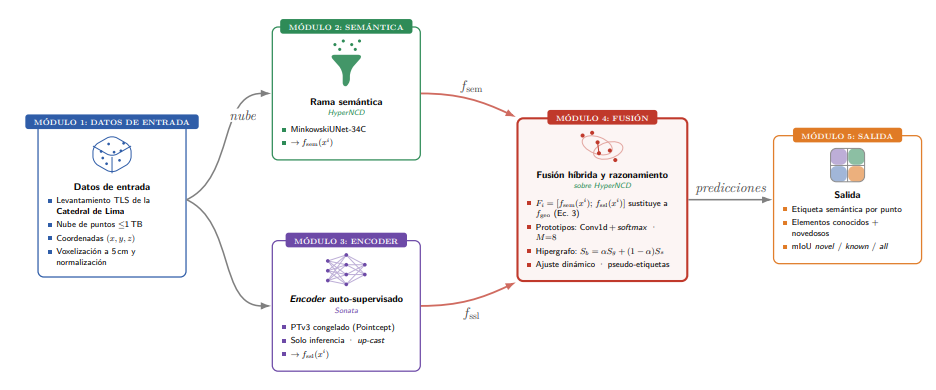
\includegraphics[width=\linewidth]{imagenes/grafico.png}
\caption{Diseño del modelo híbrido propuesto. Elaboración propia.}
\label{fig:diseno}
\end{figure}

La Figura~\ref{fig:diseno} resume el sistema en cinco módulos y se lee de
izquierda a derecha. El Módulo~1 prepara los datos; los Módulos~2 y~3 describen
cada punto de dos maneras distintas e independientes; el Módulo~4 une ambas
descripciones y razona sobre ellas; el Módulo~5 entrega el resultado. Las
flechas indican qué objeto viaja entre módulos: la nube preparada, los
descriptores $f_{\mathrm{sem}}$ y $f_{\mathrm{ssl}}$, y las predicciones. Esta
sección recorre el diagrama módulo por módulo y explica cada fórmula y cada
parámetro que aparece en él.

\subsection{Módulo 1: Datos de Entrada}

El punto de partida es el levantamiento láser terrestre de la Catedral de Lima,
una nube que puede superar el terabyte y en la que cada punto guarda sus
coordenadas $(x,y,z)$ junto con los atributos que registró el sensor. Sobre esa
nube se aplican dos operaciones antes de entregarla a las dos ramas:

\begin{itemize}\setlength{\itemsep}{2pt}
\item \textbf{Voxelización a 5\,cm.} El espacio se divide en cubos de 5\,cm de
arista y de cada cubo ocupado se conserva un único punto representante. Su
efecto es doble: reduce el número de puntos y homogeniza la densidad, que en un
levantamiento TLS es muy desigual porque las zonas cercanas al escáner reciben
muchas más mediciones que las lejanas. Un vóxel más pequeño conserva más detalle
pero aumenta el número de puntos y, con él, la memoria y el tiempo de cómputo.
\item \textbf{Normalización.} Las coordenadas y los atributos se llevan a rangos
comparables, de modo que ninguna magnitud domine el cálculo por el simple hecho
de estar expresada en una escala mayor.
\end{itemize}

La salida del módulo es la nube preparada que ambas ramas reciben como entrada
común.

\subsection{Módulo 2: Rama Semántica}

La rama semántica es una MinkowskiUNet-34C, una red convolucional que opera
sobre la rejilla dispersa y que se entrena con las clases conocidas
$\mathcal{C}_k$. Para cada punto $x^i$ entrega el descriptor
$f_{\mathrm{sem}}(x^i)$, un vector de 96 números.

Esos 96 números no son medidas físicas del edificio sino coordenadas aprendidas:
la red las ajusta durante el entrenamiento de manera que dos puntos que
pertenecen a la misma clase reciban vectores próximos entre sí y dos puntos de
clases distintas reciban vectores alejados. Esa es la razón por la que el
descriptor semántico se considera una descripción de \emph{a qué se parece} un
punto. Al tratarse de una red entrenada, su salida cambia en cada época y debe
recalcularse.

\subsection{Módulo 3: Codificador Auto-supervisado Congelado}

La segunda rama es el codificador PTv3 preentrenado por Sonata sobre unas 140
mil escenas sin etiquetas humanas. Se usa \emph{congelado}: sus pesos no se
modifican y la red se ejecuta solo en inferencia, igual que se usaría una regla
ya calibrada. Para cada punto entrega $f_{\mathrm{ssl}}(x^i)$, un vector de 1088
números, resultado de concatenar las anchuras $512+384+192$ de las tres últimas
etapas durante la propagación inversa del submuestreo (\emph{up-cast}), que
devuelve las características a la resolución de entrada.

Que el codificador esté congelado tiene dos consecuencias directas. La primera
es que su salida no depende del entrenamiento y basta calcularla una vez por
sección. La segunda es que lo que aporta al modelo es exclusivamente la
estructura aprendida durante el preentrenamiento, sin adaptarse a las clases de
este proyecto, que nunca ha visto.

\subsection{Módulo 4: Fusión Híbrida y Razonamiento}

Es el módulo donde reside el aporte de la tesis y el único que se modifica. En
él ocurren cuatro operaciones encadenadas: la concatenación de los dos
descriptores, la formación de prototipos, la construcción del hipergrafo y la
generación de pseudo-etiquetas.

\subsubsection{Concatenación de los Descriptores}

Cada punto pasa a describirse con un solo vector que reúne las dos
descripciones:
\begin{equation}
F_i=\left[f_{\mathrm{sem}}(x^i);\,f_{\mathrm{ssl}}(x^i)\right].
\label{eq:hibrido}
\end{equation}
Donde:
\begin{itemize}\setlength{\itemsep}{1pt}
\item $F_i$: descriptor compuesto del punto $i$, el vector que entra al
razonamiento.
\item $f_{\mathrm{sem}}(x^i)$: descriptor semántico del Módulo~2, 96
dimensiones.
\item $f_{\mathrm{ssl}}(x^i)$: descriptor auto-supervisado del Módulo~3, 1088
dimensiones.
\item $[\;;\;]$: concatenación, es decir, colocar un vector a continuación del
otro.
\end{itemize}

La concatenación no promedia ni mezcla los dos vectores: los deja disponibles a
la vez para el módulo siguiente. La Ec.~\eqref{eq:hibrido} sustituye a la
Ec.~\eqref{eq:hyperncd3}, que es la que emplea HyperNCD en su formulación
original. La diferencia entre ambas es el segundo componente y, con él, el
tamaño del descriptor: la línea base describe cada punto con $96+6=102$ números,
de los cuales solo 6 provienen de la forma local, mientras que el modelo
propuesto lo describe con $96+1088=1184$. Esta sustitución es la única
diferencia entre la línea base y el modelo propuesto; todo lo que viene después
permanece intacto.

\subsubsection{Formación de Prototipos}

El razonamiento no se hace punto por punto, sino sobre $K$ representantes
llamados prototipos, con $K$ igual al número de clases del conjunto. Una cabeza
convolucional unidimensional asigna a cada punto una puntuación $z_{i,k}$ por
prototipo, y una función \emph{softmax} convierte esas puntuaciones en pesos de
pertenencia:
\begin{equation}
s_{i,k}=\frac{\exp\left(z_{i,k}\right)}{\sum_{j=1}^{K}\exp\left(z_{i,j}\right)},
\qquad \sum_{k=1}^{K}s_{i,k}=1 .
\label{eq:softmax}
\end{equation}
Donde:
\begin{itemize}\setlength{\itemsep}{1pt}
\item $z_{i,k}$: puntuación que la cabeza otorga al punto $i$ para el prototipo
$k$; puede ser cualquier número real.
\item $s_{i,k}$: peso con el que el punto $i$ pertenece al prototipo $k$. Es un
valor entre 0 y 1 y el conjunto de pesos de un punto suma 1, de modo que se lee
como un reparto de pertenencia.
\item $K$: número de prototipos.
\end{itemize}

La matriz $S_p$ formada por todos los $s_{i,k}$ es la \emph{asignación suave}:
suave porque un punto no se adjudica en bloque a un único prototipo, sino que
puede pertenecer en parte a varios, lo que resulta necesario en las zonas de
transición entre elementos arquitectónicos. Cada prototipo se obtiene entonces
como el promedio de los descriptores de los puntos, ponderado por esa
pertenencia:
\begin{equation}
P_k=\frac{\sum_{i}s_{i,k}\,F_i}{\sum_{i}s_{i,k}} .
\label{eq:prototipo}
\end{equation}
El prototipo $P_k$ es, por tanto, el descriptor típico del grupo $k$. Como
$P_k$ se calcula a partir de $F_i$, la sustitución de la
Ec.~\eqref{eq:hibrido} se propaga a todo lo que sigue.

\subsubsection{Afinidad entre Prototipos e Hiperaristas}

Para relacionar los prototipos entre sí se mide su afinidad con dos criterios
complementarios. El semántico compara la dirección de los descriptores mediante
la similitud por coseno:
\begin{equation}
S_s^{(ij)}=\frac{\left\langle P_i,\;P_j\right\rangle}{\lVert P_i\rVert\;\lVert P_j\rVert},
\label{eq:coseno}
\end{equation}
que vale 1 cuando ambos vectores apuntan en la misma dirección y disminuye a
medida que se separan; compara el perfil de la descripción y no su magnitud. El
criterio geométrico compara la distancia entre descriptores mediante un núcleo
gaussiano:
\begin{equation}
S_g^{(ij)}=\exp\left(-\frac{\lVert f^{(i)}-f^{(j)}\rVert^{2}}{\tau}\right),
\label{eq:gauss}
\end{equation}
que vale 1 cuando los dos descriptores coinciden y cae hacia 0 conforme se
alejan. Donde:
\begin{itemize}\setlength{\itemsep}{1pt}
\item $\lVert f^{(i)}-f^{(j)}\rVert^{2}$: distancia al cuadrado entre los
descriptores de las regiones $i$ y $j$. En la línea base ese descriptor es
$f_{\mathrm{geo}}$, de 6 dimensiones; en el modelo propuesto es
$f_{\mathrm{ssl}}$.
\item $\tau$: temperatura, fijada en 0{,}1. Controla a qué velocidad decae la
semejanza con la distancia: un valor pequeño hace al criterio exigente, porque
solo considera afines a los prototipos muy próximos; un valor grande lo hace
permisivo.
\end{itemize}

Ambos criterios se combinan en una única medida, ya presentada en la
Ec.~\eqref{eq:afinidad}, $S_b=\alpha\,S_g+(1-\alpha)\,S_s$. El parámetro
$\alpha\in[0,1]$ reparte el peso entre los dos criterios: con $\alpha=1$ la
afinidad depende solo de la forma, con $\alpha=0$ solo de la semántica, y los
valores intermedios los mezclan. Como los dos sumandos se multiplican por pesos
que suman 1, $S_b$ permanece en el mismo rango que $S_g$ y $S_s$, lo que hace
comparables los valores obtenidos con distintos $\alpha$.

Con esa medida se construye el hipergrafo: cada prototipo se conecta con los
$M=8$ prototipos de mayor $S_b$, y ese conjunto de nueve nodos forma una
hiperarista. La diferencia con un grafo ordinario está en el número de nodos que
una relación puede abarcar. Una arista corriente une exactamente dos nodos, de
modo que para expresar que una clase novedosa se parece a la vez a varias clases
conocidas haría falta descomponer esa relación en varias comparaciones por
pares. Una hiperarista la expresa de una sola vez, y es esa concurrencia la que
permite explicar un elemento no visto en términos de los que sí se vieron. Un
valor de $M$ mayor produce hiperaristas más grandes y relaciones más difusas;
uno menor, relaciones más estrictas pero con menos contexto.

\subsubsection{Pseudo-etiquetas}

El resultado del razonamiento se convierte en pseudo-etiquetas, es decir,
etiquetas que el propio modelo asigna y que después usa como si fueran
verdaderas para seguir entrenando. Dos mecanismos las regulan:

\begin{itemize}\setlength{\itemsep}{2pt}
\item \textbf{Normalización de Sinkhorn-Knopp.} Ajusta iterativamente la matriz
de asignación hasta que sus filas y columnas sumen los valores prefijados. Su
propósito es repartir las pseudo-etiquetas de forma equilibrada entre clases y
evitar el colapso, es decir, que el modelo asigne casi todos los puntos a una
sola clase por ser la más frecuente.
\item \textbf{Suavizado de etiquetas $\epsilon=0{,}15$.} En lugar de afirmar que
un punto pertenece con certeza total a la clase ganadora, se le asigna
$1-\epsilon$ a esa clase y se reparte $\epsilon$ entre las demás. El modelo
aprende así a no confiar por completo en una etiqueta que él mismo ha generado,
lo que reduce el sobreajuste a sus propios errores.
\end{itemize}

\subsection{Módulo 5: Salida}

El sistema entrega una etiqueta semántica por punto, que puede corresponder a
una clase conocida o a una novedosa, y las métricas de la
Sección~\ref{sec:metricas}: el mIoU de la Ec.~\eqref{eq:miou} reportado por
separado sobre las clases conocidas, las novedosas y el total. Como las clases
novedosas se descubren sin nombre, antes de calcular su mIoU es necesario
decidir qué agrupación descubierta corresponde a qué clase real, lo que se
resuelve con el emparejamiento húngaro de la Ec.~\eqref{eq:hungaro}.

\subsection{Resumen de los Parámetros del Diseño}
\label{sec:parametros}

La Tabla~\ref{tab:parametros} reúne los parámetros que aparecen en el diagrama,
con su valor y con el efecto que tiene modificarlos.

\begin{table}[H]
\centering
\setstretch{1}\small
\setlength{\tabcolsep}{4pt}
\caption{Parámetros del diseño, su significado y el efecto de modificarlos.
Elaboración propia.}
\label{tab:parametros}
\begin{tabular}{@{}p{1.5cm}p{4.4cm}p{1.9cm}p{4.6cm}@{}}
\toprule
\textbf{Símbolo} & \textbf{Qué representa} & \textbf{Valor} & \textbf{Efecto de modificarlo} \\
\midrule
Vóxel & Arista del cubo con el que se submuestrea la nube & 5\,cm & Menor: más detalle y más memoria; mayor: menos puntos y pérdida de elementos finos \\
$f_{\mathrm{sem}}$ & Descriptor semántico por punto & 96 dim. & Fijado por la arquitectura de la red troncal \\
$f_{\mathrm{ssl}}$ & Descriptor auto-supervisado por punto & 1088 dim. & Fijado por las tres últimas etapas del \emph{encoder} \\
$K$ & Número de prototipos & Igual al de clases & Menor: clases distintas se mezclan; mayor: una misma clase se fragmenta \\
$\alpha$ & Peso de la componente geométrica frente a la semántica en $S_b$ & $[0,1]$, se calibra & Hacia 1 decide la forma; hacia 0 decide la semántica \\
$\tau$ & Temperatura del núcleo gaussiano & 0{,}1 & Menor: solo los prototipos muy próximos resultan afines; mayor: criterio permisivo \\
$M$ & Vecinos que forman cada hiperarista & 8 & Mayor: relaciones más amplias y difusas; menor: más estrictas y con menos contexto \\
$\epsilon$ & Suavizado de las pseudo-etiquetas & 0{,}15 & Mayor: menos confianza en la propia etiqueta; menor: riesgo de reforzar errores \\
\bottomrule
\end{tabular}
\end{table}
